% ---------
% --------
%!TEX TS-program = pdflatex
%!TEX encoding = UTF-8 Unicode
%!TEX spellcheck = English (Aspell)

\documentclass[11pt]{article}
\usepackage{lucy,handout,graphicx}
\newproof{theorem*}{Theorem}
\usepackage{fourier-orns}
\usepackage{mathtools}
\usepackage[normalem]{ulem} % either use this (simple) or
\usepackage{tikz}
\newcommand{\ulinefill}{\leavevmode\leaders\hrule height 0.4pt\hfill\kern0pt}
\pagestyle{empty}

\allowdisplaybreaks

\begin{document}

\noindent Name \underline{\hspace{12cm}}\\


\begin{center}
\LARGE\textbf{Quiz 8}%
\end{center}

\begin{enumerate}
    \item (3 points) Select all valid topological orders for the graph below.
    \begin{center}
        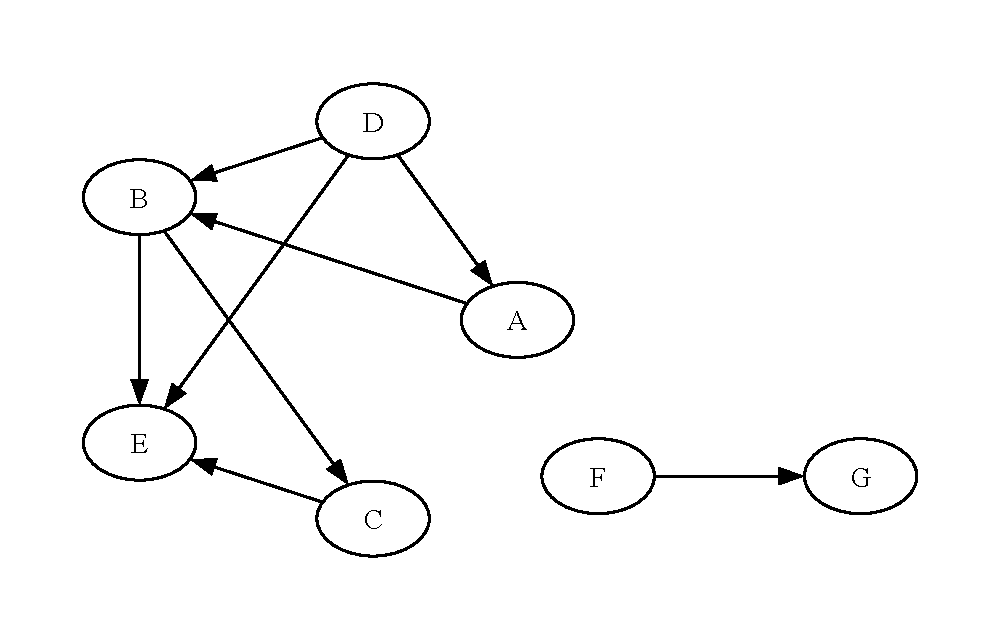
\includegraphics[width=.7\textwidth]{topo_order_graph.pdf}
    \end{center}
    \begin{itemize}
        \item $A B C D E F G$
        \item $G F E D C B A$
        \item $D A F B E C G$
        \item $F D G A B E C$
        \item $F G$
    \end{itemize}
    \item (3 points) Which type of graph has the larger number of distinct topo orders?
    \begin{itemize}
        \item A directed graph with $n$ nodes and $0$ edges
        \item A directed tree with $n$ nodes and $n-1$ edges
        \item A directed graph with $n$ nodes and $n\cdot(n+1)/2$ edges (a complete garph)
        but no cycles
    \end{itemize}
    \item (4 points) Recall the minimum coins problem from earlier in the course: \emph{Compute the minimum number
    of coins needed to make change for $n$, given that the coins are
    of denominations 1, 3, 4}. We solved this by defining a recursive definition
    for the subproblems:
    Let $MC(i)$ be the minimum number of coins needed to make change for $i$.
    Then the recursive definition is:
    \begin{equation}
        MC(i)=
    \begin{cases}
        1 & if i=1, 3, 4,\\
        2 & if i=2,\\
        1+\min\{MC(i-1),MC(i-3),MC(i-4)\} & i>0.
    \end{cases}
\end{equation}

    We have previously constructed the \emph{recursion tree} for a call
    to $MC(n)$; a recursion tree has a node for every \emph{call}
    and an edge from a call to its child calls.

    We will now construct a \emph{dependency graph} for a call to
    $MC(n)$; here, there is a node for every \emph{subproblem}
    and an edge from subproblem $u$ to subproblem $v$ if evaluating
    $u$ depends on the answer to $v$.

    For example, evaluating $MC(n)$ depends on $MC(n-1)$, so there should be a directed edge
    from $MC(n)$ to $MC(n-1)$ in the dependency graph.

    \begin{enumerate}
        \item 
    Fill in all of the edges in this example (assume no nodes are base cases):

    \begin{center}
    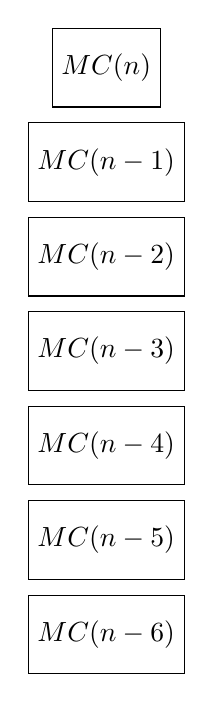
\begin{tikzpicture}[
        every node/.style={draw, minimum size=10mm}
    ]
        \node at (0, 0) {$MC(n)$};
        \node at (0, -1.2) {$MC(n-1)$};
        \node at (0, -2.4) {$MC(n-2)$};
        \node at (0, -3.6) {$MC(n-3)$};
        \node at (0, -4.8) {$MC(n-4)$};
        \node at (0, -6.0) {$MC(n-5)$};
        \node at (0, -7.2) {$MC(n-6)$};
    \end{tikzpicture}
    \end{center}
    \item Now consider memoizing this recursion into an array $M$.
    We know we can fill $M$ from left to right, but now let's think
    about filling it in an order determined by some graph structure
    in the dependency graph $G$. Fill in the blank:

    We fill $M$ in a \underline{\hspace{2in}} of $G$.
\end{enumerate}


    \item There are only four more weeks in the semester and it's time to make sure
    you have the best chance to get the grades you want!
    If you anticipate needing or wanting to attend office hours
    before the semester ends, whether to redo quizzes/homeworks or to get
    help with course material or exam prep, please
    write down any additional times you would like to request and I will do my best
    to add them to the current schedule (Mon 11-12, Fri 9-10).
    

\end{enumerate}



\end{document}
